\iffalse
\subsubsection{Controllers}
\begin{figure}[H]
  \centering
  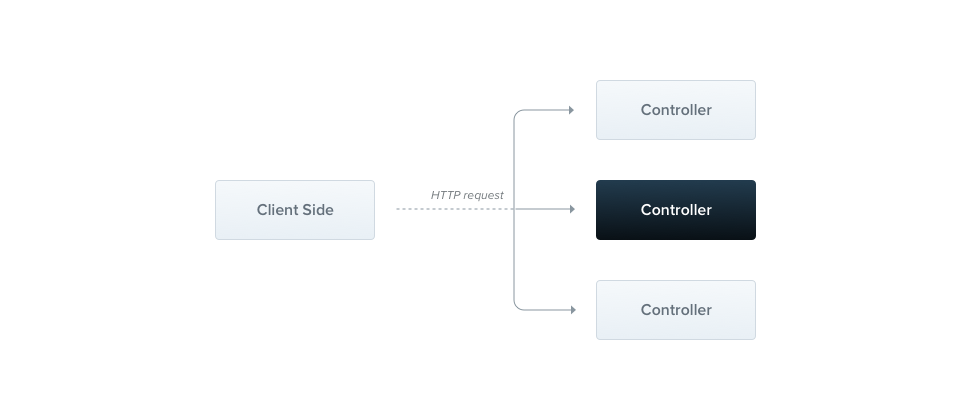
\includegraphics[width=0.8\textwidth]{./assets/p2/Controllers_1.png}
\end{figure}

A controller's purpose is to receive specific requests for the application.
The routing mechanism controls which controller receives which requests.
Frequently, each controller has more than one route, and different routes can perform different actions.

\subsubsection{Providers}
\begin{figure}[H]
  \centering
  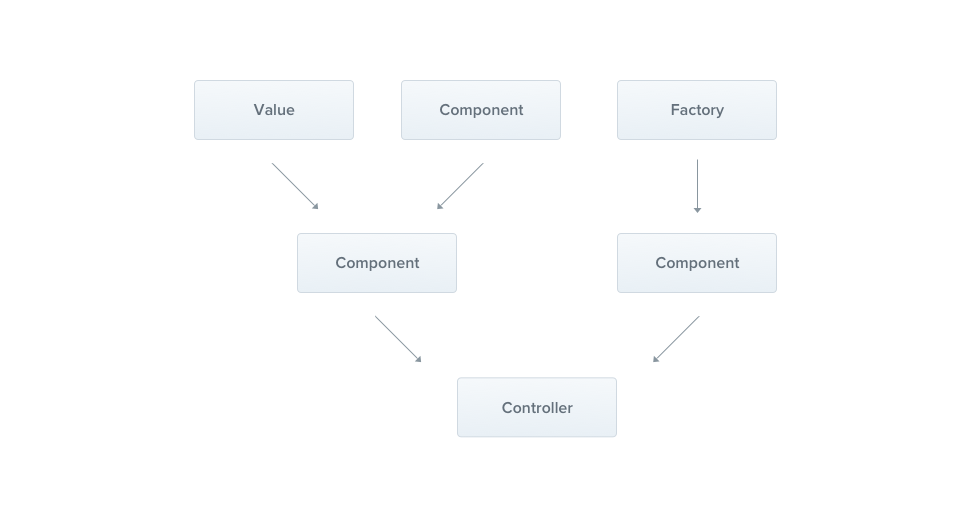
\includegraphics[width=0.8\textwidth]{./assets/p2/Providers_1.png}
\end{figure}

Nest introduces a new concept called providers.
Many of the basic Nest classes may be treated as a provider --- services, repositories, factories, helpers, and so on.
The main idea of a provider is that it can be injected as dependency; this means objects can create various relationships with each other, and the function of ``wiring up'' instances of objects can largely be delegated to the Nest runtime system.

\subsubsection{Modules}
\begin{figure}[H]
  \centering
  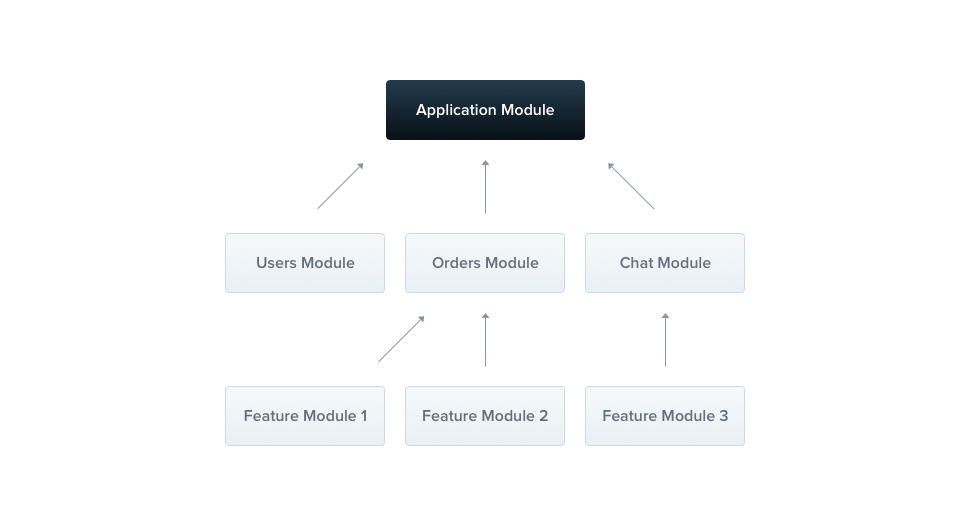
\includegraphics[width=0.8\textwidth]{./assets/p2/Modules_1.png}
\end{figure}

Each application has at least one module, a root module.
The root module is the starting point Nest uses to build the application graph --- the internal data structure Nest uses to resolve module and provider relationships and dependencies.

While very small applications may theoretically have just the root module, this is not the typical case.
We want to emphasize that modules are strongly recommended as an effective way to organize your components.
Thus, for most applications, the resulting architecture will employ multiple modules, each encapsulating a closely related set of capabilities.

The module encapsulates providers by default. This means that it's impossible to inject providers that are neither directly part of the current module nor exported from the imported modules. Thus, you may consider the exported providers from a module as the module's public interface, or API\@.
\fi
